
% 微分方程的数值方法

\chapter{BEM数值方法}

\section{假设和引理}

\begin{assumption}\label{unique}
	在这一章节中, 我们令$-\infty\leq\alpha<\beta\leq\infty$,并且假设时间变换的SDE\cref{basic SDE}在$(\alpha,\beta)\subseteq\mathbb{R}$有唯一强解,即:$$\mathbb{P}(x(t)\in(\alpha,\beta), t\geq0)=1.$$
\end{assumption}
\begin{assumption}\label{monotony}
	在这一章节中, 我们令$c\in[-\infty,+\infty),I=(c,+\infty),\operatorname{}d\in I$是区间中任意的一点, 并且假设SDE\cref{basic SDE}的漂移项系数$f$满足下述单调性 :
	\begin{equation}
		f:I\to\mathbb{R}  , 使得 \exists K \in\mathbb{R},\forall x,y\in I,x\leq y,f(y)-f(x)\leq K(y-x).
	\end{equation}
\end{assumption}

\begin{assumption}\label{super linear growth}
	在这一章节中, 我们假设SDE\cref{basic SDE}的漂移项系数$f$满足线性增长条件, 即存在一个常数$K>0$, 使得:
	\begin{equation}
		|f(x)| \le K(1+|x|). 
	\end{equation}
\end{assumption}
对于SDE\cref{basic SDE}在漂移项系数$f$在单调条件下, 解的存在唯一性的证明可以参考\cite{umarov2018beyond}中漂移性满足全局Lipschitz条件的证明.
\section{强收敛性}
对于随机微分方程\cref{basic SDE},它的BEM数值格式是:
\begin{equation}\label{eq:1}
	X_{t_{i+1}}=X_{t_i}+f(X_{t_{i+1}})\Delta E_{i}+\sigma\Delta B_{E_{i}},\quad i=0,1,2,\ldots,\qquad X_0=X(0)
\end{equation}
其中$\Delta E_{i}=E(t_{i+1})-E(t_i)$以及$\Delta B_{E_{i}}=B(E{(t_{i+1})})-B(E({t_i}))$.
\begin{theorem}\label{main th}
	对于任意的$\epsilon>0$,令$\epsilon < T1 < T2$,在\cref{moment}, \cref{unique},\cref{monotony}和\cref{super linear growth}的条件下,存在常数C,使得下面的不等式成立:
	$$\mathbb{E}\left[\sup\limits_{i=\lceil T_1/\Delta t \rceil\ldots \lceil T_2/\Delta t \rceil. } |X({t_i})-X_{t_i}|\right]\le C\Delta t^\alpha.$$
\end{theorem}
\begin{proof}
	由于第一变量变换和第二变量变换公式\cref{first},\cref{second}的成立,使得我们可以考虑\cref{basic SDE}在$[t_i,t_{i+1})$的积分:
	\begin{align}
		\int_{t_i}^{t_{i+1}}dX(s)=\int_{t_i}^{t_{i+1}}f(X(s))dE(s)+\int_{t_i}^{t_{i+1}}\sigma dB(E(s))
	\end{align}
	等价于
	\begin{align}
		\int_{t_i}^{t_{i+1}}dX(s))=\int_{E_{t_i}}^{E_{t_{i+1}}}f(X(D(s-)))ds+\int_{E_{t_i}}^{E_{t_{i+1}}}\sigma dB(s)
	\end{align}
	针对于漂移项$f(X(D(s-)))$,下面等式恒成立:
	\begin{align}\label{eq:ito}
		\int_{E(t_i)}^{E(t_{i+1})} f(X(D(t_{i+1}-)))) - f(X(D(t-))) dt = \int_{E(t_i)}^{E(t_{i+1})} \int^{D(t_{i+1}-)}_{D(t-)} df(X(s)) dt
	\end{align}
	对于$df(X(s))$,由\cref{ito}的时间变换It\^{o}公式:
	\begin{align*}
		\begin{gathered}
			f(X(t))-f(0)=\int_{0}^{E(t)}f(X(D(s-)))f^{\prime}\left(X(D(s-))\right)+\frac{\sigma^{2}}{2}f^{\prime\prime}\big(X(D(s-))\big)ds \\
			+\int_{0}^{E(t)}\sigma f^{\prime}\big(X(D(s-))\big)dB(s)
		\end{gathered}
	\end{align*}
	于是\cref{eq:ito}变成
	\begin{equation}\label{eq:ito1}
		\begin{aligned}
			&\quad\int_{E(t_i)}^{E(t_{i+1})} f(X(D(t_{i+1}-))) - f(X(D(t-))) dt \\
			&= \int_{E(t_i)}^{E(t_{i+1})} \int_{t}^{t_{i+1}} \left( f(X(D(s))) f^{\prime}(X(D(s))) + \frac{1}{2} \sigma^2 f^{\prime\prime}(X(D(s))) \right) ds \, dt\\
			&\quad + \int_{E(t_i)}^{E(t_{i+1})} \int_{t}^{t_{i+1}} \sigma f^{\prime}(X(D(s))) \, dB(s) \, dt .
		\end{aligned}
	\end{equation}
	由\cref{basic SDE}与\cref{eq:ito1},以及\cite[Theorem 3.1]{kobayashi2011stochastic}可以得到
	\begin{align*}
		X(t_{i+1}) 
		&= X(t_i) + \int_{E(t_i)}^{E(t_{i+1})} f(X({D(t_{i+1})})) \, dt + \int_{t_i}^{t_{i+1}} \sigma \, dB(E(t)) \\
		&\quad + \int_{E(t_i)}^{E(t_{i+1})} \int_{t}^{t_{i+1}}\left( f(X(D(s))) f^{\prime}(X(D(s))) + \frac{1}{2} \sigma^2 f^{\prime\prime}(X(D(s))) \right) ds \, dt \\
		&\quad + \int_{E(t_i)}^{E(t_{i+1})} \int_{t}^{t_{i+1}}\sigma f^{\prime}(X(D(s)))) \, dB(s) \, dt \\
		&= X(t_i) + \int_{t_i}^{t_{i+1}} f(X({t_i)}) \, dE(t) + \int_{t_i}^{t_{i+1}} \sigma \, dB(E(t)) \\
		&\quad + \int_{t_i}^{t_{i+1}} \int_{E(t)}^{E(t_{i+1})} \left( f(X(D(s))) f^{\prime}(X(D(s))) + \frac{1}{2} \sigma^2 f^{\prime\prime}(X(D(s))) \right) ds \, dE(t) \\
		&\quad + \int_{t_i}^{t_{i+1}} \int_{E(t)}^{E(t_{i+1})}\sigma f^{\prime}(X(D(s))) \, dB(s) \, dE(t)\\
		&= X(t_i) + \int_{t_i}^{t_{i+1}} f(X({t_i})) \, dE(t) + \int_{t_i}^{t_{i+1}} \sigma \, dB(E(t)) \\
		&\quad + \int_{t_i}^{t_{i+1}} \int_{t}^{t_{i+1}} \left( f(X(s)) f^{\prime}(X(s)) + \frac{1}{2} \sigma^2 f^{\prime\prime}(X(s)) \right) dE(s) \, dE(t) \\
		&\quad + \int_{t_i}^{t_{i+1}} \int_{t}^{t_{i+1}}\sigma f^{\prime}(X(s)) \, dB(E(s)) \, dE(t)
	\end{align*}
	因此
	\begin{align}\label{eq:2}
		X(t_{i+1})
		&= X(t_i) + \int_{t_i}^{t_{i+1}} f(X({t_{i+1})}) \, dE(t) + \int_{t_i}^{t_{i+1}} \sigma \, dB(E(t)) + R_i
	\end{align}
	其中
	\begin{align*}
		R_i = &-\int_{t_i}^{t_{i+1}} \int_{t}^{t_{i+1}} \left( f(X(s)) f^{\prime}(X(s)) + \frac{1}{2} \sigma^2 f^{\prime\prime}(X(s)) \right) dE(s) \, dE(t)\\
		&-\int_{t_i}^{t_{i+1}} \int_{t}^{t_{i+1}} \sigma f^{\prime}(X(s)) \, dB(E(s)) \, dE(t)
	\end{align*}
	将$R_i$分解成$R_i = R_i^{(1)} + R_i^{(2)}$,其中:
	\begin{align*}
		& R_s^{(1)} = -\int_{t_i}^{t_{i+1}} \int_{t}^{t_{i+1}} \left( f(X(s)) f^{\prime}(X(s)) + \frac{1}{2} \sigma^2 f^{\prime\prime}(X(s)) \right) dE(s) \, dE(t).\\
		& R_s^{(2)} = -\int_{t_i}^{t_{i+1}} \int_{t}^{t_{i+1}} \sigma f^{\prime}(X(s)) \, dB(E(s)) \, dE(t)  
	\end{align*}
	和离散格式相减,即\cref{eq:2}-\cref{eq:1}得到:
	\begin{equation}
		X({t_{i+1}})-X_{t_{i+1}}=X({t_i})-X_{t_i}+(f{(X({t_{i+1}}))}-f{(X_{t_{i+1}})})\Delta E_{i}+R_{i}
	\end{equation}
	令$e_i = X({t_i})-X_{t_i}$
	由\cref{monotony}得到:
	\begin{equation}
		(1-K_1\Delta E_s)e_{s+1}\leq e(s)+R_{s},\quad\text{其中}s=\lceil T1/\Delta t \rceil,\lceil T1/\Delta t \rceil+1 \ldots \lceil T2/\Delta t \rceil
	\end{equation}
	定义$\gamma_l = 1-K_1\Delta E_l$,$N_1 = \lceil T1/\Delta t \rceil$以及$N_2 = \lceil T2/\Delta t \rceil$, 在\cite{li2023convergence}, 我么可以得到对于离散后的随机过程$E_t$, 存在与$\Delta t$无关的C使得$\Delta E_t \le C \Delta t$, 所以
	\begin{equation}\label{bound}
	\sup\limits_{k=\lceil T_1/\Delta t \rceil\ldots \lceil T_2/\Delta t \rceil}	\prod\limits_{l=N_1}^{k}\gamma_l^{-1} <\sup\limits_{k=\lceil T_1/\Delta t \rceil\ldots \lceil T_2/\Delta t \rceil}	\prod\limits_{l=N_1}^{k}(1-C\Delta t)^{-1}
	\end{equation}
	通过对$\Delta t$取极限, 于是
	\[
	\sup\limits_{k=\lceil T_1/\Delta t \rceil\ldots \lceil T_2/\Delta t \rceil}	\prod\limits_{l=N_1}^{k}\gamma_l^{-1} <\infty
	\]
	由\cref{gronwall}结合\cref{bound},我们可以得到
	$$\mathbb{E}  \left[\sup\limits_{k=\lceil T_1/\Delta t \rceil\ldots \lceil T_2/\Delta t \rceil}|e_k|\right] \leq C\mathbb{E}\sum\limits_{j=N_1}^{N_2}\left|R_{j}^{(1)} \right| + C\mathbb{E}\sum\limits_{j=N_1}^{N_2}\left|R_{j}^{(2)} \right|.$$
	
	由于$f$满足单调条件和超线性增长条件, 因此$f$的导数在有限区间必然是有界的. 
	于是对于第一项,  由\cref{main pro}和\cref{main lemma}可以推导出类似的性质和引理, 于是可以得到
	\begin{align*}
		\mathbb{E} \left[|R_{j+1}^{(1)}| \right] &= \mathbb{E}_D \left[
		\int_{t_i}^{t_{i+1}} \int_{t_i}^{t}  \mathbb{E}_B \left( f(X(s)) f^{\prime}(X(s)) + \frac{1}{2} \sigma^2 f^{\prime\prime}(X(s)) \right) dE(s) \, dE(t)
		\right] \\
		&= C\mathbb{E}_D \left[
		\int_{t_i}^{t_{i+1}} \int_{t_i}^{t}  \mathbb{E}_B \left[1+|X(s)|^a \right] dE(s) \, dE(t)
		\right] \\
		& \le C\mathbb{E}_D \left[
		\int_{t_i}^{t_{i+1}} \int_{t_i}^{t}  1 dE(s) \, dE(t)
		\right] \\
		&\le C\Delta t^{1+\alpha}. 
	\end{align*}
	于是
	\begin{equation}
		\sum\limits_{N_1}^{N_2}\mathbb{E}\left|R_{j}^{(1)}\right| \leq
		C\sum\limits_{j=N_1}^{N_2}\Delta t^{1+\alpha} \le C\Delta t^\alpha
	\end{equation}
	因为
	\begin{align*}
		\mathbb{E}\left[ R_{k}^{(2)}|\mathcal{F}_{k\Delta t} \right] &= \mathbb{E}_D\mathbb{E}_B\left[ \int_{t_i}^{t_{i+1}} \int_{t_i}^{t} \sigma f^{\prime}(X(s)) \, dB(E(s)) \, dE(t) \right]\\
		&=\mathbb{E}_D\left[ \int_{t_i}^{t_{i+1}} \mathbb{E}_B\int_{t_i}^{t} \sigma f^{\prime}(X(s)) \, dB(E(s)) \, dE(t) \right]\\
		&= 0
	\end{align*}
	因此
	\begin{align*}
		\sum_{j=N_1}^{N_2}R_{j}^{(2)} 
	\end{align*}
	是鞅.我们知道由BDG不等式和\cref{main lemma}可以得到:
	\begin{equation*}
		\mathbb{E}[dB_EdE]^2=\mathbb{E}[(dB_E)^2(dE)^2]=\mathbb{E}_D[(dE)^2\mathbb{E}_B(dB_E)^2]\leq
		C\mathbb{E}_{D}[dE]^3\leq C\Delta t ^{1+2\alpha}
	\end{equation*}
	于是对于第二项, 
	\begin{align*}
		\mathbb{E} \left[|R_{j+1}^{(2)}| \right] &= \mathbb{E}_D \left[
		\int_{t_i}^{t_{i+1}} \mathbb{E}_B  \left[\int_{t_i}^{t}  \sigma f^{\prime}(X(s)) dB_{E(s)}\right] \, dE(t)
		\right] \\
		& \le C\mathbb{E}_D \left[
		\int_{t_i}^{t_{i+1}} \left[\int_{t_i}^{t}  \mathbb{E}_B\left(\sigma f^{\prime}(X(s))\right)^2 dE(s)\right]^{\frac{1}{2}} \, dE(t)
		\right] \\
		&\le C \mathbb{E}_D 
		\int_{t_i}^{t_{i+1}} \left[\int_{t_i}^{t}  1 dE(s)\right]^{\frac{1}{2}} \, dE(t)\\
		&\le C\Delta t^{\frac{1}{2}+\alpha}. 
	\end{align*}
	
	由BDG不等式和Cauchy-Schwarz不等式,可以得到:
	\begin{equation*}
		\mathbb{E}\sum_{j=N_1}^{N_2}\left|R_{j}^{(2)}\right|  \le C\mathbb{E} \left|\sum_{j=N_1}^{N_2}(R_{j}^{(2)})^2\right|^{\frac{1}{2}} \le C\sqrt{\sum_{j=N_1}^{N_2}\mathbb{E}(R_{j}^{(2)})^2}
		\le C\sqrt{\sum_{j=N_1}^{N_2}\Delta t^{1+2\alpha}} \le C\Delta t^{\alpha}
	\end{equation*}
	综上所述,
	\begin{equation*}
		\mathbb{E} [e_n] \leq C\Delta t^\alpha
	\end{equation*}
\end{proof}
%	tips:We have also proved that $\mathbb{E} [\Delta E \Delta B_E ] \le C\Delta t ^{1+\frac{\alpha}{2}}$,however it seems that it's nothing help here.

\section{数值模拟}

\begin{example}
	考虑时间变换的的布朗运动驱动的CIR过程
    \begin{equation}\label{CIR}
        dy(t)=\kappa(\theta-y(t))dE(t)+\sigma\sqrt{y(t)}dB(E(t)),\quad t\geq0,\quad y(0)>0.
    \end{equation}
\end{example}
如果 $2\kappa\theta\geq\sigma^{2}$, 那么 $D=(0,\infty)$ 并且\cref{unique} 在 $(\alpha,\beta)=$
$(0,\infty)$是成立的. 
另外, 使用It\^{o}公式$X(t)=F((y(t))$,其中$F$是由\cref{Lamperti}定义,即对时间变换的CIR过程进行Lamperti变换可以得到
\begin{equation}
	dX(t)=f(X(t))dE(t)+\frac12\sigma dB(E(t)),\quad t\geq0,\quad X(0)=\sqrt{y(0)}
\end{equation}
其中
\begin{equation}
	f(X)=\dfrac{1}{2}\kappa\left(\theta_vX^{-1}-X\right),\quad X>0
\end{equation}
其中 $\theta_v=\theta-\frac{\sigma^2}{4\kappa}$ ,并且 BEM数值格式如下
\begin{equation}
	X_{t_{i+1}}=X_{t_{i}}+f(X_{t_{i+1}})\Delta E_i+\frac{1}{2}\sigma\Delta B_{E_i},\quad k=0,1,\dots 
\end{equation}
观察到
\begin{equation}
	f'(X)=-\frac{1}{2}\kappa(\theta_vX^{-2}+1)
\end{equation}
以及
\begin{equation}
	f(X)f'(X)+\frac{\sigma^2}{2}f''(X)=-\frac{\kappa^2}{4}(\theta_v^2X^{-3}-X)+\frac{1}{2}\kappa\theta_vX^{-3}\sigma^2.
\end{equation}
因此为了满足\cref{moment},只需要满足
\begin{equation}
	\sup_{0\leq t\leq T}\mathbb{E}[X(t)^{-3}]=\sup_{0\leq t\leq T}\mathbb{E}[y(t)^{-\frac{3}{2}}] < \infty.
\end{equation}
对于时间变换的CIR过程y(t)的矩有界,即
\begin{equation}
	\sup\limits_{0\leq t\leq T}\mathbb{E}[y(t)^q]<\infty\quad\mathrm{for}\quad q>-\frac{2k\theta}{\sigma^2},
\end{equation}
下面验证,对于由时间变换的的布朗运动驱动的CIR过程\cref{CIR}的精确解矩有界.
\begin{proposition}
	对于由时间变换的布朗运动驱动的CIR过程\cref{CIR},其中$y_0>0$,$1<p<\frac{2K\theta}{\sigma^2}-1$,都存在一个常数C使得
	\begin{equation*}
		\sup\limits_{t\in[0,T]}\mathbb{E}\left[\left(y(t)\right)^{-p}\right]\leq C(1+y(0)^{-p})
	\end{equation*}
\end{proposition}
\begin{proof}
	定义停时$\tau_{n}=\mathrm{inf}\{0<s\leq T;y(s)\leq1/n\}$,通过It\^{o}公式,我们可以得到
	$$\begin{aligned}
		\mathbb{E}_B\left[(y(t\wedge\tau_{n}))^{-p}\right] &=y(0)^{-p}-p\mathbb{E}_B\left[\int_{0}^{t\wedge\tau_{n}}\frac{K(\theta-y(s))}{(y(s))^{p+1}}dE(s)\right]\\
		&+p(p+1)\frac{\sigma^{2}}{2}\mathbb{E}_B\left[\int_{0}^{t\wedge\tau_{n}}\frac{1}{(y(s))^{p+1}}dE(s)\right] \\
		&\leq y(0)^{-p}+pK\int_{0}^{t}\mathbb{E}_B\left(\frac{1}{(y(s\wedge\tau_{n}))^{p}}
		\right)dE(s) \\
		&+\mathbb{E}_B\left[\int_0^{t\wedge\tau_n}\frac{p\left(\frac{(p+1)\sigma^2}{2}-K\theta\right)}{(y(s))^{p+1}}dE(s)\right]
	\end{aligned}$$
	通过计算可以找到正数$\underline C$使得, 当$\frac{(p+1)\sigma^2}{2}-K\theta<0$时,对于任意的 $y(0)=x>0$,都有
	$$\frac{p\left(\frac{(p+1)\sigma^2}{2}-K\theta\right)}{x^{p+1}}\leq \underline C$$
	因此
	$$\mathbb{E}_B\left[(y(t\wedge\tau_n))^{-p}\right]\leq y(0)^{-p}+\underline{C}E(T)+pK\int_0^t\sup_{r\in[0,s]}\mathbb{E}_B\left[(y(r\wedge\tau_n))^{-p}\right]dE(s)$$
	于是由Gronwall不等式,可以得到
	$$\sup\limits_{t\in[0,T]}\mathbb{E}_B\left[(y(t\wedge\tau_n)^x)^{-p}\right]\leq\left(y(0)^{-p}+\underline{C}E(T)\right)\exp(pKE(T))$$
	两边同时取$\mathbb{E}_D$并使用Cauchy-Schwarz不等式,得到
	$$\begin{aligned}
		\sup\limits_{t\in[0,T]}\mathbb{E}\left[(y(t\wedge\tau_n)^x)^{-p}\right]&\leq\mathbb{E}\left[\left(y(0)^{-p}+\underline{C}E(T)\right)\exp(pKE(T))\right]\\
		&\leq\sqrt{\mathbb{E}\left[\left(y(0)^{-p}+\underline{C}E(T)\right)^2\right]\mathbb{E}\left[\exp(2pKE(T))\right]}
	\end{aligned}$$
	从\cite{jum2014strong}可以得到
	\begin{equation}
		\mathbb{E}[E^n(t)]=\frac{n!}{\Gamma(n\alpha+1)}t^{n\alpha}
	\end{equation}
	\begin{equation}
		\mathbb{E}[e^{\lambda E(t)}]<\infty
	\end{equation}
	其中$\lambda \in \mathbb{R},t>0$.最后,让 $n\to+\infty$,我们完成了这个证明.
\end{proof}
\begin{remark}
	在这里只是证明了当$1<p<\frac{2K\theta}{\sigma^2}-1$的时候,矩的存在性,实际上更可以证明$p<\frac{2K\theta}{\sigma^2}$,但是证明起来过于复杂,这里就不在说明,对于我们的结果已经够用了.
\end{remark}
对于\cref{moment},可以验证只需要保证$1 < \frac{4}{3}\frac{k\theta}{\sigma^2}$成立即可,而这个区间可以被$1<p<\frac{2K\theta}{\sigma^2}-1$包含在内,因此只需要保证p在后者这个区间即可.至于\cref{monotony},在$(0,\infty)$中很容易可以验证存在这样的$\kappa$使之成立.因此由\cref{main th}可以得到,对于时间变换的CIR过程,使用BEM数值格式的强收敛阶是$\alpha$.

在我们的数值实验中,我们关注端点$T = 1$处的$L_1$误差,因此我们令
\begin{align*}
	e_T^{i}=\mathbb{E}\left|X_T^{\delta _{15}}-X_T^{\delta _i}\right|
\end{align*}
其中$X_T^{\delta _i}$是步长为$\delta _i$时T处的模拟值,$\delta _i = 2^{-i}$,对于我们的数值实验,取$\theta=0.125,\kappa=2$以及$\sigma=0.5$,采用蒙德卡洛方法,
\begin{align*}
	e_{T}^i\approx\frac{1}{10^3}\sum_{j=1}^{10^3}\left|X_T^{\delta _{15}}-X_T^{\delta _i}\right|.
\end{align*}
选择步长为$2^{-15}$作为参考,通过${2^{-11},2^{-10},2^{-9},2^{-8}}$的步长来估计$L_1$误差.

\begin{example}
	考虑时间变换的的布朗运动驱动的CEV过程
    \begin{equation}\label{CEV}
    	dy(t)=\kappa(\theta-y(t))dE(t)+\sigma y(t)^\alpha dB_{E(t)}
    \end{equation}
\end{example}

其中 $0.5<\alpha<1,\kappa,\theta,\sigma>0.$ 通过变换$X(t)=F(y(t))$的变换之后,其中$F$是由\cref{Lamperti}定义,我们可以得到\cref{monotony}在$(\alpha,\beta)=(0,\infty)$下,是成立的,此时	$$dX(t)=f(X(t))dE(t)+(1-\alpha)\sigma dB(E(t))$$
其中
$$f(X)=(1-\alpha)\left(\kappa\theta X^{-\frac\alpha{1-\alpha}}-\kappa X-\frac{\alpha\sigma^2}2X^{-1}\right),\quad X>0.$$
同时我们需要验证另一个\cref{moment}.因为 $\alpha>0.5$, 于是$\frac{1}{1-\alpha}>2$,因此
$$f^{\prime}(X)=-\alpha\kappa\theta X^{-\frac1{1-\alpha}}-(1-\alpha)\kappa+(1-\alpha)\frac{\alpha\sigma^2}2X^{-2},\quad X>0$$
同时我们又有
$$f^{\prime\prime}(X)=\frac\alpha{1-\alpha}\kappa\theta X^{-\frac{2-\alpha}{1-\alpha}}-(1-\alpha)\alpha\sigma^2X^{-3}.$$
下面验证,对于由时间变换的的布朗运动驱动的CEV过程\cref{CEV}的精确解矩有界.
\begin{proposition}
	对于由时间变换的布朗运动驱动的CEV过程\cref{CEV},其中$X_0>0$,对于任意的$\frac{1}{2}<\alpha<1$和任意的$p>0$,都存在一个常数C使得
	\begin{equation*}
		\sup\limits_{t\in[0,T]}\mathbb{E}\left[\left(y(t)\right)^{-p}\right]\leq C(1+y(0)^{-p})
	\end{equation*}
\end{proposition}
\begin{proof}
	定义停时$\tau_{n}=\mathrm{inf}\{0<s\leq T;y(s)\leq1/n\}$,通过It\^{o}公式,我们可以得到
	$$\begin{aligned}
		\mathbb{E}_B\left[(y(t\wedge\tau_{n}))^{-p}\right] &=y(0)^{-p}-p\mathbb{E}_B\left[\int_{0}^{t\wedge\tau_{n}}\frac{K(\theta-y(s))}{(y(s))^{p+1}}dE(s)\right]\\
		&+p(p+1)\frac{\sigma^{2}}{2}\mathbb{E}_B\left[\int_{0}^{t\wedge\tau_{n}}\frac{1}{(y(s))^{p+2(1-\alpha)}}dE(s)\right] \\
		&\leq y(0)^{-p}+pK\int_{0}^{t}\mathbb{E}_B\left(\frac{1}{(y(s\wedge\tau_{n}))^{p}}
		\right)dE(s) \\
		&+\mathbb{E}_B\left[\int_0^{t\wedge\tau_n}\left(p(p+1)\frac{\sigma^2}{2}\frac{1}{(y(s))^{p+2(1-\alpha)}}-p\frac{K\theta}{(y(s))^{p+1}}\right)dE(s)\right]
	\end{aligned}$$
	可以找到正数$C$使得, 对于任意的 $y(0)=x>0$,都有
	$$\left(p(p+1)\frac{\sigma^2}{2}\frac{1}{x^{p+2(1-\alpha)}}-p\frac{K\theta}{x^{p+1}}\right)\leq C$$
	通过计算可以得到,$\underline C=p(2\alpha-1)\frac{\sigma^2}{2}\left[(p+2(1-\alpha))\frac{\sigma^2}{2K\theta}\right]^{\frac{p+2(1-\alpha)}{2\alpha-1}}$ 是最小的上界. 因此
	$$\mathbb{E}_B\left[(y(t\wedge\tau_n))^{-p}\right]\leq y(0)^{-p}+\underline{C}E(T)+pK\int_0^t\sup_{r\in[0,s]}\mathbb{E}_B\left[(y(r\wedge\tau_n))^{-p}\right]dE(s)$$
	于是由Gronwall不等式,可以得到
	$$\sup\limits_{t\in[0,T]}\mathbb{E}_B\left[(y(t\wedge\tau_n)^x)^{-p}\right]\leq\left(y(0)^{-p}+\underline{C}E(T)\right)\exp(pKE(T))$$
	两边同时取$\mathbb{E}_D$并使用Cauchy-Schwarz不等式,得到
	$$\begin{aligned}
		\sup\limits_{t\in[0,T]}\mathbb{E}\left[(y(t\wedge\tau_n)^x)^{-p}\right]&\leq\mathbb{E}\left[\left(y(0)^{-p}+\underline{C}E(T)\right)\exp(pKE(T))\right]\\
		&\leq\sqrt{\mathbb{E}\left[\left(y(0)^{-p}+\underline{C}E(T)\right)^2\right]\mathbb{E}\left[\exp(2pKE(T))\right]}
	\end{aligned}$$
	从\cite{jum2014strong}可以得到
	\begin{equation}
		\mathbb{E}[E^n(t)]=\frac{n!}{\Gamma(n\alpha+1)}t^{n\alpha}
	\end{equation}
	\begin{equation}
		\mathbb{E}[e^{\lambda E(t)}]<\infty
	\end{equation}
	其中$\lambda \in \mathbb{R},t>0$.最后,让 $n\to+\infty$,我们完成了这个证明.
\end{proof}


由Lamperti变换可知,$X(t)$的逆阶矩可以$y(t)$的逆阶矩控制,于是\cref{moment}成立.因此根据\cref{main th}可以得到由时间变换布朗运动驱动的CEV过程的收敛阶是$\alpha$
\

\begin{figure}[htp!]
	\centering
	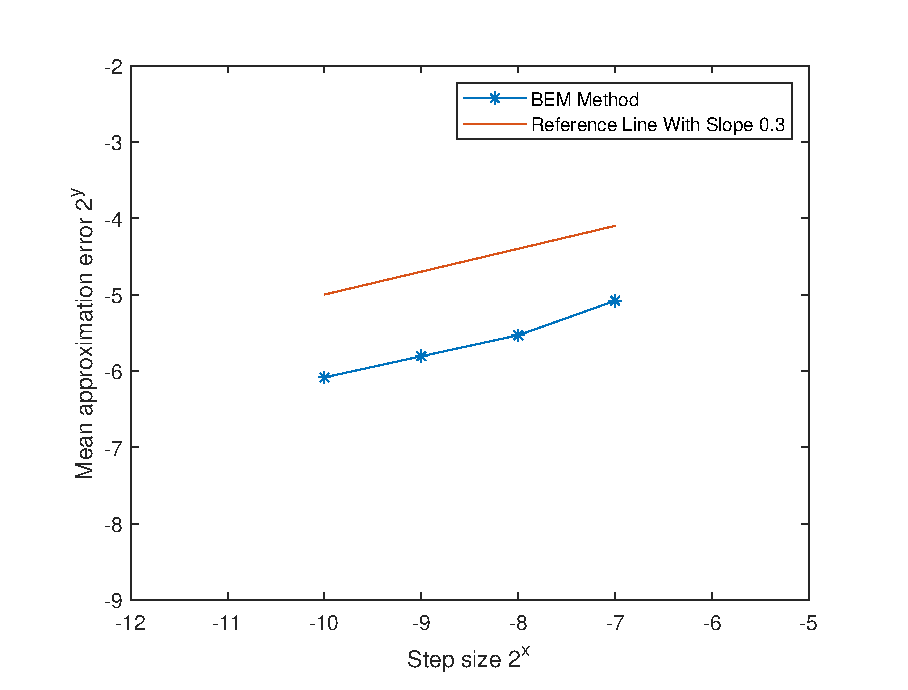
\includegraphics[width=0.45\linewidth]{BEMalpha=0.3.eps}
	\hfill
	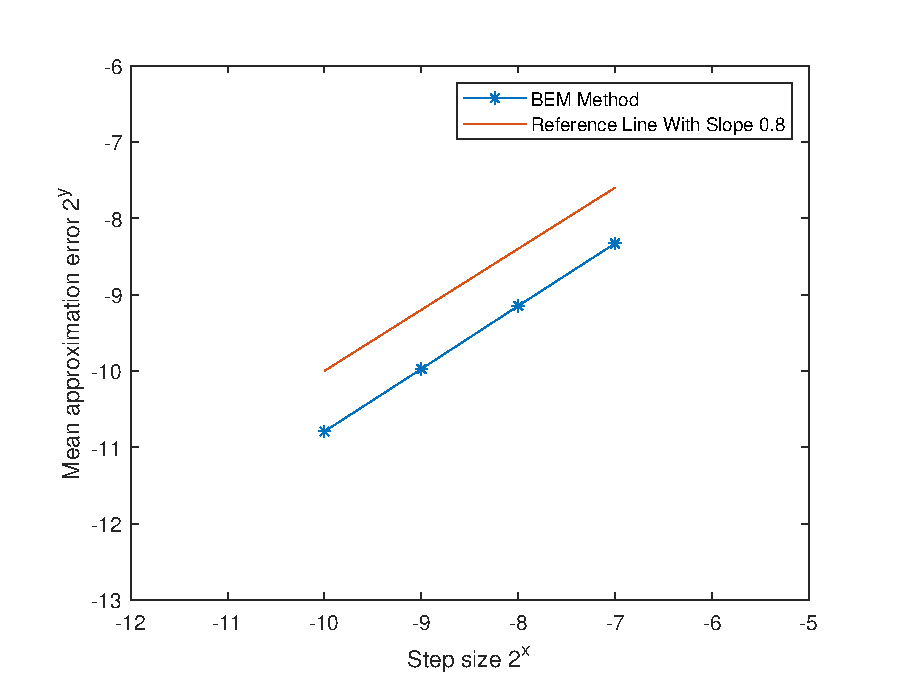
\includegraphics[width=0.45\linewidth]{BEMalpha=0.8.eps}
	\caption{时间变换CIR过程的数值解与解析解之间的绝对误差估计.左图是$\alpha=0.3$,右图是$\alpha=0.8$}
	\label{fig:image}
	\vspace{-2ex}
\end{figure}


\section{关于1阶的写在这里}


\begin{assumption}
	假设下面不等式成立:
	$|f' f(x)| + |\sigma f'| + |\sigma F''| \leq K(1 + |x|);$
\end{assumption}

\begin{theorem}
	设 $X$ 为随机微分方程 (3.1) 的解,假设条件 $\mathcal{H}_1, \mathcal{H}_2$ 和 $\mathcal{H}_4$ 满足。
	设 $X^{\delta}$ 为在 (4.3)–(4.4) 中定义的 Euler-Maruyama 型近似过程。则存在与 $\delta$ 无关的常数 $C > 0$,使得对所有 $\delta \in (0,1)$,
	\[
	\mathbb{E} \left[ \sup_{0 \leq s \leq T} | X_s - X_s^\delta | \right] \leq C \delta。
	\]
	因此,$X^\delta$ 在 $[0, T]$ 上以 1 阶一致强收敛于 $X$。
\end{theorem}

\begin{proof}
	
	利用 (3.1) 并通过 Itô 公式展开 $\mathrm{d}E_r$ 积分的被积函数,
	
	$$
	\begin{aligned}
		X_{\tau_{n+1}} &= X_{\tau_n} +  \int_{\tau_n}^{\tau_{n+1}} f(X_{\tau_n}) \, \mathrm{d}E_r + \int_{\tau_n}^{\tau_{n+1}} \sigma \, \mathrm{d}B_{E_r} + R_{(\tau_n, \tau_{n+1})}; \\
		R_{(a,b)} &:=  \int_a^b \int_a^{r_2} \left( f(X_{\tau_{n_{r_1}}})f'(X_{\tau_{n_{r_1}}}) + \frac{\sigma ^2}{2} f''(X_{\tau_{n_{r_1}}})  \right) \, \mathrm{d}E_{r_1} \, \mathrm{d}E_{r_2} + \int_a^b \int_a^{r_2} \sigma f'(X_{\tau_{n_{r_1}}})   \, \mathrm{d}B_{E_{r_1}} \, \mathrm{d}E_{r_2},
	\end{aligned}
	$$
	因此:
	$Z_t := \sup_{0 \leq s \leq t} | X_s - {X_s^\delta} | \leq I_1 + I_2 $,其中
	
	$$
	\begin{aligned}
		&I_1 := \sup_{0 \leq s \leq t} \left| \int_0^s F(X_{\tau_{n_r}}) - F(X_{\tau_{n_r}}^\delta)  \, \mathrm{d}E_r \right|; \\
		&I_2 := \sup_{0 \leq s \leq t} \left| \sum_{i=0}^{n_s - 1} R_{(\tau_{t}, \tau_{t+1})} + R_{(\tau_{n_s}, s)} \right|.
	\end{aligned}
	$$
	很容易观察到
	\begin{equation}\label{I1}
		\mathbb{E}_B[I_1] \leq C \int_0^t \mathbb{E}_B[Z_r] \, \mathrm{d}E_r.
	\end{equation}
	
	主要的技术部分涉及余项 $I_2$,其中包含两个不同的双重积分:$\mathrm{d}E_{r_1} \, \mathrm{d}E_{r_2}$ 和 $\mathrm{d}B_{E_{r_1}} \, \mathrm{d}E_{r_2}$。我们将在下面逐一处理这些积分。
	
	对于第一个积分$ \mathrm{d}E_{r_1} \, \mathrm{d}E_{r_2}$,
	\begin{align}
		& \quad \mathbb{E}_B \left[\sup_{0 \leq s \leq t} \left| \int_0^s \int_{\tau_{n_2}}^{r_2} ff'  + \frac{\sigma^2}{2} f'' \, \mathrm{d}E_{r_1} \, \mathrm{d}E_{r_2} \right|\right] \nonumber \\
		&\leq  \frac{3}{2}K \mathbb{E}_B[Y_T^{(1)}] \int_0^t \int_{\tau_{n_{r_2}}}^{r_2} \, \mathrm{d}E_{r_1} \, \mathrm{d}E_{r_2} \nonumber \\
		&\leq  \frac{3}{2}K E_T \mathbb{E}_B[Y_T^{(1)}] \delta.  \label{I21}
	\end{align}
	
	另一方面,我们需要估计 $\mathbb{E}_B \left[\sup_{0 \leq s \leq t} |M_{n_s} + U_s|\right]$,其中 $M_0 := 0$,对于 $n \geq 1$,$M_n := \sum_{i=0}^{n-1} L_i$,
	$$
	L_i := \int_{\tau_i}^{\tau_{i+1}} \int_{\tau_i}^{r_2} \sigma f' \, \mathrm{d}B_{E_{r_1}} \, \mathrm{d}E_{r_2}, \quad U_s := \int_{\tau_{n_s}}^s \int_{\tau_{n_s}}^{r_2} \sigma f' \, \mathrm{d}B_{E_{r_1}} \, \mathrm{d}E_{r_2}.
	$$
	
	我们首先验证随机积分 $L_i, i=0,1,\ldots,n_t-1$ 关于 $\mathbb{P}_B$ 是不相关的。令 $i < j$,因此 $\tau_{i+1} \leq \tau_j$。观察到 $\mathbb{E}_B [L_i L_j] = \mathbb{E}_B \left[L_i \mathbb{E}_B [L_j | \mathcal{F}_{E_{\tau_j}}]\right]$。根据假设和估计 (3.4),
	
	$$
	\mathbb{E}_B \left[\int_{\tau_j}^{\tau_{j+1}} \left|\int_{\tau_j}^{r_2} F_x G( X_{r_1}) \, \mathrm{d}B_{E_{r_1}}\right|^2 \mathrm{d}E_{r_2}\right] \leq \delta^2 K^2 \mathbb{E}_B [Y_t^{(2)}] < \infty.
	$$
	
	因此,$\mathbb{E}_B \left[L_j | \mathcal{F}_{E_{\tau_j}}\right] = \int_{\tau_j}^{\tau_{j+1}} \mathbb{E}_B \left[\int_{\tau_j}^{r_2} F_x G(X_{r_1}) \, \mathrm{d}B_{E_{r_1}} | \mathcal{F}_{E_{\tau_j}}\right] \mathrm{d}E_{r_2} = 0$,这是由于条件 Fubini 定理(参考文献 [26] 中的定理 27.17)和鞅性质,从而得到不相关性。另一方面,由于 $E$ 具有连续路径,变量变换公式(参考文献 [13] 中的定理 3.1)表明 $M_n$ 可以表示为
	
	$$
	\sum_{i=0}^{n-1} \int_{i\delta}^{(i+1)\delta} \int_{i\delta}^{E_{r_2}} \sigma f' \, \mathrm{d}B_{r_1} \, \mathrm{d}r_2。
	$$
	
	该表示式,以及参考文献 [12] 中引理 5.7.1 和 10.8.1 的证明,表明离散时间过程 $(M_n)_{n \geq 0}$ 是一个平方可积的 $((\mathcal{F}_{n\delta})_{n \geq 0}, \mathbb{P}_B)$-鞅,初始值为 0。因此,由 BDG 不等式 (3.2) 和 $L_i$ 的不相关性,
	
	$$
	\mathbb{E}_B \left[\sup_{0 \leq s \leq t} M_{n_s}^2\right] \leq b_2 \sum_{i=0}^{n_t-1} \mathbb{E}_B [L_i^2]。
	$$
	因此,由 Cauchy-Schwartz 不等式,
	\begin{align}
		\mathbb{E}_B\left[\sup_{0\leq s\leq t}M_{n_s}^2\right] 
		&\leq b_2\delta\sum_{i=0}^{n_t-1}\int_{\tau_i}^{\tau_{i+1}}\mathbb{E}_B
		\left[\int_{\tau_i}^{r_2}\left|\sigma f'\right|^2\mathrm{d}E_{r_1}\right]
		\mathrm{d}E_{r_2} \nonumber \\
		&\leq2b_2\delta K^2\mathbb{E}_B[Y_T^{(2)}]\sum_{i=0}^{n_t-1}\int_{\tau_i}^
		{\tau_{i+1}}(E_{r_2}-E_{\tau_i})\mathrm{d}E_{r_2} \nonumber \\
		&\leq 2b_2E_TK^2\mathbb{E}_B[Y_T^{(2)}]\delta^2. \label{I221}
	\end{align}
	另一方面, 
	\begin{align}
		\mathbb{E}_B\left[\sup_{0\leq s\leq t}U_s^2\right]  
		&\leq\mathbb{E}_B\biggl[\sup_{0\leq s\leq t}(E_s-E_{\tau_{n_s}})\int_{\tau_{n_s}}^s\left|\int_{\tau_{n_s}}^{r_2}\sigma f'\mathrm{d}B_{E_{r_1}}\right|^2\mathrm{d}E_{r_2}\biggr] \nonumber \\ &\leq\delta\int_0^t\mathbb{E}_B\left[\sup_{s\in[r_2,t]}\left|\int_{\tau_{n_s}}^{r_2}\sigma f'\mathrm{d}B_{E_{r_1}}\right|^2\right]\mathrm{d}E_{r_2}.\label{I222}
	\end{align}
	由于$\{(\tau_{n_s},r_2)~:~r_2~\leq~s~\leq~t\}~\subset~\{(\tau_{n_{r_2}},u)~:~\tau_{n_{r_2}}~\leq~u~\leq~r_2\},$于是
	\begin{align*}
		&\quad\mathbb{E}_B\Big[\sup_{S\in[r_2,t]}\Big|\int_{\tau_x}^{r_2}\sigma f'\mathrm{d}B_{E_{r_1}}\Big|^2\Big]  \\
		&\le \mathbb{E}_B\left[\sup_{u\in[\tau_{n_{r_2}},r_2]}\left|\int_{\tau_{n_{r_2}}}^u\sigma f'\mathrm{d}B_{E_{r_1}}\right|^2\right] \\
		&\leq b_2\mathbb{E}_B\left[\int_{\tau_{n_{r_2}}}^{r_2}\left|\sigma f'\right|^2\mathrm{d}E_{r_1}\right]\\
		&\leq 2b_2K^2\mathbb{E}_B[Y_T^{(2)}]\delta.
	\end{align*}
	因此,\cref{I222}的上界为  $2b_2E_TK^2\mathbb{E}_B[Y_T^{(2)}]\delta^2.$ 将其与 \cref{I221} 结合得:
	\begin{equation}\label{I22}
		\mathbb{E}_B\left[\sup_{0\leq s\leq t}|M_{n_s}+U_s|^2\right] 
		\leq 8b_2E_TK^2\mathbb{E}_B[Y_T^{(2)}]\delta^2. 
	\end{equation}
	根据估计 \cref{I21} 和 \cref{I22},
	\begin{equation}\label{I2}
		\mathbb{E}_B[I_2] 
		\leq \left\{\frac{3}{2}E_T\mathbb{E}_B[Y_T^{(1)}]+(8b_2E_T\mathbb{E}_B[Y_T^{(2)}])^{1/2}\right\}K\delta. 
	\end{equation}
	
	现在,将 \cref{I1}和 \cref{I2}与  $\mathbb{E}_B[Y_T^{(1)}]\leq\sqrt{2}\mathbb{E}_B[Y_T^{(2)}]^{1/2}$ 结合得:
	\begin{equation*}
		\mathbb{E}_B[Z_t] 
		\leq \xi_2(E_T)\mathbb{E}_B[Y_T^{(2)}]^{1/2}\delta + K\int_0^t\mathbb{E}_B[Z_r] \mathrm{d}E_r.
	\end{equation*}
	
	其中 $\xi_2(u) := K(\frac{3\sqrt{2}}{2}u + (8b_2u)^{1/2}).$
	应用 Gronwall 类型不等式, 对两边取 $ \mathbb{E}_D $并使用 Cauchy-Schwartz 不等式得 
	\begin{equation*}
		\mathbb{E}[Z_T] \leq \mathbb{E}[\xi_2^4(E_T)]^{1/4}\mathbb{E}[(Y_T^{(2)})^2]^{1/4}\mathbb{E}[e^{2KE_T}]^{1/2}\delta.
	\end{equation*}
	由于对于任意的$\lambda>0, t>0,n>0$, 都有$\mathbb{E}[e^{\lambda E_t}] < \infty$, 以及$\mathbb{E}[E^n(t)] < \infty$, 再结合\cref{main pro}, 于是可以得到该定理成立.
	
	
	
	
	
\end{proof}